\subsection{Pengujian Gerakan Linier dan Estimasi Posisi pada \emph{Real Robot}}
\label{subsec:linierrobot}

Pengujian gerakan linier dan estimasi posisi pada \emph{real robot} dilakukan dengan cara yang sama dengan yang dilakukan di simulasi seperti yang ada di bagian \ref{subsec:liniersimulasi}.
Perbedaannya, pada pengujian ini komponen navigasi yang sebelumnya berasal dari simulasi digantikan dengan \emph{navigation node} yang mengakses perangkat yang ada pada \emph{real robot}.
Seperti yang terlihat pada gambar \ref{fig:rosgraphnavigation},
  \emph{node} \lstinline{/move_for} akan mengirimkan \emph{topic} \lstinline{/cmd_vel} dengan fungsi yang sama ke \emph{node} \lstinline{/navigation},
  setelah itu \emph{node} \lstinline{/odometry_echo} akan menerima \emph{topic} \lstinline{/odom} yang berasal dari \emph{node} \lstinline{/navigation}.

\begin{figure}[ht]
  \centering
  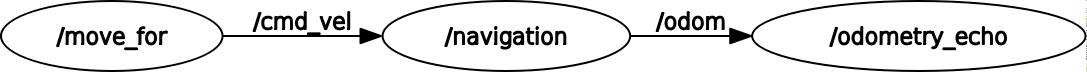
\includegraphics[width=0.95\textwidth,keepaspectratio]{gambar/rosgraph-navigation.png}
  \caption{Relasi antar-\emph{node} dari pengujian gerakan linier dan estimasi posisi pada \emph{real robot}.}
  \label{fig:rosgraphnavigation}
\end{figure}

Pengujian pada \emph{real robot} ini juga dilakukan dengan berbagai macam konfigurasi kecepatan X dan Y yang diperintahkan selama 3 detik.
Hasil pengujian ini bisa dilihat pada tabel \ref{tb:gerakanlinierrobot}.
Pada tabel tersebut, nilai yang ada di kolom \emph{speed} adalah besar kecepatan yang diatur pada \emph{topic} \lstinline{/cmd_vel},
  nilai yang ada di kolom \emph{estimated position} didapatkan dari perkalian besar kecepatan dengan durasi pengujian,
  nilai yang ada di kolom \emph{measured position} didapatkan dari pengukuran perpindahan \emph{real robot} menggunakan meter ukur,
  dan terakhir nilai yang ada di kolom \emph{odometry position} didapatkan dari data yang ada di \emph{topic} \lstinline{/odom}.

\begin{sidewaystable}
  \centering
  \caption{Hasil estimasi posisi dari gerakan linier pada \emph{real robot} selama 3 detik.}
  \label{tb:gerakanlinierrobot}
  \begin{tabular}{|c|c|c|c|c|c|c|c|c|}
    \hline \rowcolor[HTML]{E0E0E0}
    \multicolumn{2}{|c|}{\textbf{Speed}} &
    \multicolumn{2}{|c|}{\textbf{Expected Position}} &
    \multicolumn{2}{|c|}{\textbf{Measured Position}} &
    \multicolumn{3}{|c|}{\textbf{Odometry Position}}
    \\ \hline \rowcolor[HTML]{E0E0E0}
    \textbf{X (m/s)} & \textbf{Y (m/s)} &
    \textbf{X (m)} & \textbf{Y (m)} &
    \textbf{X (m)} & \textbf{Y (m)} &
    \textbf{X (m)} & \textbf{Y (m)} & \textbf{Error}
    \csvreader[head to column names]{data/gerakan_linier_robot.csv}{}{
      \\ \hline
      \speedx & \speedy &
      \expectedx & \expectedy &
      \measuredx & \measuredy &
      \odometryx & \odometryy & \odometryerror
    }
    \\ \hline
  \end{tabular}
\end{sidewaystable}


Seperti kesimpulan pada pengujian sebelumnya,
  dari data yang dihasilkan oleh pengujian ini juga dapat diketahui bahwa gerakan yang diperintahkan robot cenderung menghasilkan posisi robot yang sesuai dengan posisi perkiraan (\emph{estimated position}).
Lebih lanjut, ketika hasil tersebut ditampilkan sebagai grafik,
  seperti yang terlihat pada gambar \ref{fig:grafikgerakanlinierrobot},
  hasil yang didapatkan juga cenderung memiliki arah positif dan negatif yang sesuai dengan yang diharapkan (\emph{expected}) walaupun dengan \emph{error} jarak yang relatif tidak kecil terutama pada posisi di sumbu X yang seharusnya bernilai 0.


\begin{figure} [ht]
  \centering
  \begin{tikzpicture}
    \begin{axis}[
        height=0.45\textwidth,
        width=0.8\textwidth,
        ylabel=X (meter),
        xticklabels={,,},
        ymajorgrids,
        bar width=3pt,
        ybar=0pt,
        xmin=-1,
        xmax=12,
      ]
      \addplot table[x=index,y=expectedx,col sep=comma]{data/gerakan_linier_robot.csv};
      \addplot table[x=index,y=measuredx,col sep=comma]{data/gerakan_linier_robot.csv};
      \addplot table[x=index,y=odometryx,col sep=comma]{data/gerakan_linier_robot.csv};
    \end{axis}
  \end{tikzpicture}
  \begin{tikzpicture}
    \begin{axis}[
        height=0.45\textwidth,
        width=0.8\textwidth,
        ylabel=Y (meter),
        xticklabels={,,},
        legend style={
          at={(0.5,-0.2)},
          anchor=north,
          legend columns=-1,
        },
        ymajorgrids,
        bar width=3pt,
        ybar=0pt,
        xmin=-1,
        xmax=12,
      ]
      \addplot table[x=index,y=expectedy,col sep=comma]{data/gerakan_linier_robot.csv};
      \addplot table[x=index,y=measuredy,col sep=comma]{data/gerakan_linier_robot.csv};
      \addplot table[x=index,y=odometryy,col sep=comma]{data/gerakan_linier_robot.csv};
      \legend{Expected,Measured,Odometry}
    \end{axis}
  \end{tikzpicture}
  \caption{Grafik estimasi posisi dari gerakan linier pada \emph{real robot}.}
  \label{fig:grafikgerakanlinierrobot}
\end{figure}

